\documentclass[twoside]{book}

% Packages required by doxygen
\usepackage{fixltx2e}
\usepackage{calc}
\usepackage{doxygen}
\usepackage{graphicx}
\usepackage[utf8]{inputenc}
\usepackage{makeidx}
\usepackage{multicol}
\usepackage{multirow}
\PassOptionsToPackage{warn}{textcomp}
\usepackage{textcomp}
\usepackage[nointegrals]{wasysym}
\usepackage[table]{xcolor}

% Font selection
\usepackage[T1]{fontenc}
\usepackage{mathptmx}
\usepackage[scaled=.90]{helvet}
\usepackage{courier}
\usepackage{amssymb}
\usepackage{sectsty}
\renewcommand{\familydefault}{\sfdefault}
\allsectionsfont{%
  \fontseries{bc}\selectfont%
  \color{darkgray}%
}
\renewcommand{\DoxyLabelFont}{%
  \fontseries{bc}\selectfont%
  \color{darkgray}%
}
\newcommand{\+}{\discretionary{\mbox{\scriptsize$\hookleftarrow$}}{}{}}

% Page & text layout
\usepackage{geometry}
\geometry{%
  a4paper,%
  top=2.5cm,%
  bottom=2.5cm,%
  left=2.5cm,%
  right=2.5cm%
}
\tolerance=750
\hfuzz=15pt
\hbadness=750
\setlength{\emergencystretch}{15pt}
\setlength{\parindent}{0cm}
\setlength{\parskip}{0.2cm}
\makeatletter
\renewcommand{\paragraph}{%
  \@startsection{paragraph}{4}{0ex}{-1.0ex}{1.0ex}{%
    \normalfont\normalsize\bfseries\SS@parafont%
  }%
}
\renewcommand{\subparagraph}{%
  \@startsection{subparagraph}{5}{0ex}{-1.0ex}{1.0ex}{%
    \normalfont\normalsize\bfseries\SS@subparafont%
  }%
}
\makeatother

% Headers & footers
\usepackage{fancyhdr}
\pagestyle{fancyplain}
\fancyhead[LE]{\fancyplain{}{\bfseries\thepage}}
\fancyhead[CE]{\fancyplain{}{}}
\fancyhead[RE]{\fancyplain{}{\bfseries\leftmark}}
\fancyhead[LO]{\fancyplain{}{\bfseries\rightmark}}
\fancyhead[CO]{\fancyplain{}{}}
\fancyhead[RO]{\fancyplain{}{\bfseries\thepage}}
\fancyfoot[LE]{\fancyplain{}{}}
\fancyfoot[CE]{\fancyplain{}{}}
\fancyfoot[RE]{\fancyplain{}{\bfseries\scriptsize Generated on Sun Jan 25 2015 01\+:36\+:19 for Flock You! by Doxygen }}
\fancyfoot[LO]{\fancyplain{}{\bfseries\scriptsize Generated on Sun Jan 25 2015 01\+:36\+:19 for Flock You! by Doxygen }}
\fancyfoot[CO]{\fancyplain{}{}}
\fancyfoot[RO]{\fancyplain{}{}}
\renewcommand{\footrulewidth}{0.4pt}
\renewcommand{\chaptermark}[1]{%
  \markboth{#1}{}%
}
\renewcommand{\sectionmark}[1]{%
  \markright{\thesection\ #1}%
}

% Indices & bibliography
\usepackage{natbib}
\usepackage[titles]{tocloft}
\setcounter{tocdepth}{3}
\setcounter{secnumdepth}{5}
\makeindex

% Hyperlinks (required, but should be loaded last)
\usepackage{ifpdf}
\ifpdf
  \usepackage[pdftex,pagebackref=true]{hyperref}
\else
  \usepackage[ps2pdf,pagebackref=true]{hyperref}
\fi
\hypersetup{%
  colorlinks=true,%
  linkcolor=blue,%
  citecolor=blue,%
  unicode%
}

% Custom commands
\newcommand{\clearemptydoublepage}{%
  \newpage{\pagestyle{empty}\cleardoublepage}%
}


%===== C O N T E N T S =====

\begin{document}

% Titlepage & ToC
\hypersetup{pageanchor=false,
             bookmarks=true,
             bookmarksnumbered=true,
             pdfencoding=unicode
            }
\pagenumbering{roman}
\begin{titlepage}
\vspace*{7cm}
\begin{center}%
{\Large Flock You! }\\
\vspace*{1cm}
{\large Generated by Doxygen 1.8.8}\\
\vspace*{0.5cm}
{\small Sun Jan 25 2015 01:36:19}\\
\end{center}
\end{titlepage}
\clearemptydoublepage
\tableofcontents
\clearemptydoublepage
\pagenumbering{arabic}
\hypersetup{pageanchor=true}

%--- Begin generated contents ---
\chapter{Hierarchical Index}
\section{Class Hierarchy}
This inheritance list is sorted roughly, but not completely, alphabetically\+:\begin{DoxyCompactList}
\item \contentsline{section}{Audio}{\pageref{class_audio}}{}
\item \contentsline{section}{Boid}{\pageref{class_boid}}{}
\item \contentsline{section}{State}{\pageref{class_state}}{}
\begin{DoxyCompactList}
\item \contentsline{section}{Game}{\pageref{class_game}}{}
\end{DoxyCompactList}
\item \contentsline{section}{State\+Manager}{\pageref{class_state_manager}}{}
\item \contentsline{section}{Texture}{\pageref{class_texture}}{}
\item \contentsline{section}{Vec2}{\pageref{struct_vec2}}{}
\end{DoxyCompactList}

\chapter{Class Index}
\section{Class List}
Here are the classes, structs, unions and interfaces with brief descriptions\+:\begin{DoxyCompactList}
\item\contentsline{section}{\hyperlink{class_audio}{Audio} \\*Creates a \hyperlink{class_audio}{Audio} object to handle the S\+D\+L\+\_\+\+Mixer }{\pageref{class_audio}}{}
\item\contentsline{section}{\hyperlink{class_boid}{Boid} \\*Creates an \hyperlink{class_boid}{Boid} object Creates an \hyperlink{class_boid}{Boid} object that is to be used for each \hyperlink{class_boid}{Boid} }{\pageref{class_boid}}{}
\item\contentsline{section}{\hyperlink{class_game}{Game} \\*Creates an \hyperlink{class_game}{Game} object that inherits \hyperlink{class_state}{State} Creates an \hyperlink{class_game}{Game} object that inherits \hyperlink{class_state}{State} and runs the \hyperlink{class_game}{Game}. D\+I\+S\+C\+L\+A\+M\+E\+R\+: Created using Pseudo code from \href{https://www.macs.hw.ac.uk/~dwcorne/Teaching/Boids%20Pseudocode.htm}{\tt https\+://www.\+macs.\+hw.\+ac.\+uk/$\sim$dwcorne/\+Teaching/\+Boids\%20\+Pseudocode.\+htm} }{\pageref{class_game}}{}
\item\contentsline{section}{\hyperlink{class_state}{State} \\*Creates a \hyperlink{class_state}{State} object. Creates a \hyperlink{class_state}{State} object to be inherited }{\pageref{class_state}}{}
\item\contentsline{section}{\hyperlink{class_state_manager}{State\+Manager} \\*Creates a \hyperlink{class_state_manager}{State\+Manager} object. Creates a \hyperlink{class_state_manager}{State\+Manager} object to be inherited }{\pageref{class_state_manager}}{}
\item\contentsline{section}{\hyperlink{class_texture}{Texture} \\*Creates a \hyperlink{class_texture}{Texture} for use with a renderer Creates a \hyperlink{class_texture}{Texture} from an image file, this can then be used with a renderer }{\pageref{class_texture}}{}
\item\contentsline{section}{\hyperlink{struct_vec2}{Vec2} \\*Creates an \hyperlink{struct_vec2}{Vec2} structure with functions Creates an \hyperlink{struct_vec2}{Vec2} structure with overloaded operators to create a new variable type for use as a 2\+D vector }{\pageref{struct_vec2}}{}
\end{DoxyCompactList}

\chapter{Class Documentation}
\hypertarget{class_audio}{\section{Audio Class Reference}
\label{class_audio}\index{Audio@{Audio}}
}


Creates a \hyperlink{class_audio}{Audio} object to handle the S\+D\+L\+\_\+\+Mixer.  




{\ttfamily \#include $<$audio.\+h$>$}



Collaboration diagram for Audio\+:
\nopagebreak
\begin{figure}[H]
\begin{center}
\leavevmode
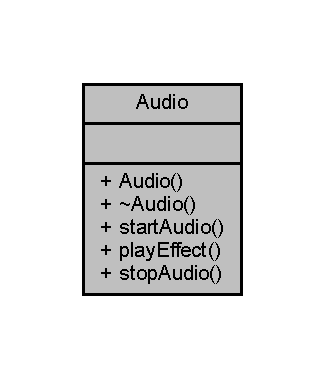
\includegraphics[width=156pt]{class_audio__coll__graph}
\end{center}
\end{figure}
\subsection*{Public Member Functions}
\begin{DoxyCompactItemize}
\item 
\hyperlink{class_audio_ae1900ee0e5254fe0c96e0b423ea02777}{Audio} (std\+::string, bool)
\item 
\hyperlink{class_audio_ae8f54deecb5f48511aaab469e80294d6}{$\sim$\+Audio} ()
\item 
void \hyperlink{class_audio_a15f1ea89039f6dbbb2260bb34f9dabdd}{start\+Audio} ()
\item 
void \hyperlink{class_audio_aea41cc6feaed4b1ab5957ea499509f55}{play\+Effect} ()
\item 
void \hyperlink{class_audio_a5d73ae24c80b37df5f167016de9c9296}{stop\+Audio} ()
\end{DoxyCompactItemize}


\subsection{Detailed Description}
Creates a \hyperlink{class_audio}{Audio} object to handle the S\+D\+L\+\_\+\+Mixer. 

\subsection{Constructor \& Destructor Documentation}
\hypertarget{class_audio_ae1900ee0e5254fe0c96e0b423ea02777}{\index{Audio@{Audio}!Audio@{Audio}}
\index{Audio@{Audio}!Audio@{Audio}}
\subsubsection[{Audio}]{\setlength{\rightskip}{0pt plus 5cm}Audio\+::\+Audio (
\begin{DoxyParamCaption}
\item[{std\+::string}]{file, }
\item[{bool}]{music}
\end{DoxyParamCaption}
)}}\label{class_audio_ae1900ee0e5254fe0c96e0b423ea02777}
Constructs an \hyperlink{class_audio}{Audio} object Constructs the \hyperlink{class_audio}{Audio} object. 
\begin{DoxyParams}{Parameters}
{\em std\+::string} & the file to be loaded \\
\hline
{\em bool} & is it a music file? if false its a sound file \\
\hline
\end{DoxyParams}
\hypertarget{class_audio_ae8f54deecb5f48511aaab469e80294d6}{\index{Audio@{Audio}!````~Audio@{$\sim$\+Audio}}
\index{````~Audio@{$\sim$\+Audio}!Audio@{Audio}}
\subsubsection[{$\sim$\+Audio}]{\setlength{\rightskip}{0pt plus 5cm}Audio\+::$\sim$\+Audio (
\begin{DoxyParamCaption}
{}
\end{DoxyParamCaption}
)}}\label{class_audio_ae8f54deecb5f48511aaab469e80294d6}
De-\/constructs a \hyperlink{class_audio}{Audio} object De-\/constructs the \hyperlink{class_audio}{Audio} object 

\subsection{Member Function Documentation}
\hypertarget{class_audio_aea41cc6feaed4b1ab5957ea499509f55}{\index{Audio@{Audio}!play\+Effect@{play\+Effect}}
\index{play\+Effect@{play\+Effect}!Audio@{Audio}}
\subsubsection[{play\+Effect}]{\setlength{\rightskip}{0pt plus 5cm}void Audio\+::play\+Effect (
\begin{DoxyParamCaption}
{}
\end{DoxyParamCaption}
)}}\label{class_audio_aea41cc6feaed4b1ab5957ea499509f55}
Plays the sound Plays the sound effect \hypertarget{class_audio_a15f1ea89039f6dbbb2260bb34f9dabdd}{\index{Audio@{Audio}!start\+Audio@{start\+Audio}}
\index{start\+Audio@{start\+Audio}!Audio@{Audio}}
\subsubsection[{start\+Audio}]{\setlength{\rightskip}{0pt plus 5cm}void Audio\+::start\+Audio (
\begin{DoxyParamCaption}
{}
\end{DoxyParamCaption}
)}}\label{class_audio_a15f1ea89039f6dbbb2260bb34f9dabdd}
Starts the \hyperlink{class_audio}{Audio} playing Starts the \hyperlink{class_audio}{Audio} playing, also checks if not playing and starts again \hypertarget{class_audio_a5d73ae24c80b37df5f167016de9c9296}{\index{Audio@{Audio}!stop\+Audio@{stop\+Audio}}
\index{stop\+Audio@{stop\+Audio}!Audio@{Audio}}
\subsubsection[{stop\+Audio}]{\setlength{\rightskip}{0pt plus 5cm}void Audio\+::stop\+Audio (
\begin{DoxyParamCaption}
{}
\end{DoxyParamCaption}
)}}\label{class_audio_a5d73ae24c80b37df5f167016de9c9296}
Stops the \hyperlink{class_audio}{Audio} playing 

The documentation for this class was generated from the following files\+:\begin{DoxyCompactItemize}
\item 
Flock You!/audio.\+h\item 
Flock You!/audio.\+cpp\end{DoxyCompactItemize}

\hypertarget{class_boid}{\section{Boid Class Reference}
\label{class_boid}\index{Boid@{Boid}}
}


Creates an \hyperlink{class_boid}{Boid} object Creates an \hyperlink{class_boid}{Boid} object that is to be used for each \hyperlink{class_boid}{Boid}.  




{\ttfamily \#include $<$boid.\+h$>$}



Collaboration diagram for Boid\+:\nopagebreak
\begin{figure}[H]
\begin{center}
\leavevmode
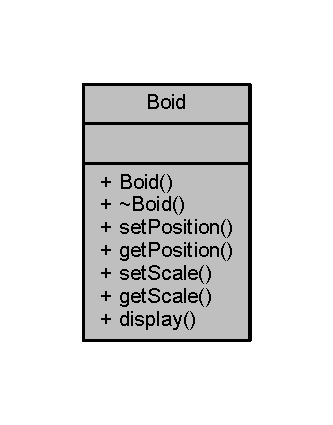
\includegraphics[width=160pt]{class_boid__coll__graph}
\end{center}
\end{figure}
\subsection*{Public Member Functions}
\begin{DoxyCompactItemize}
\item 
\hyperlink{class_boid_aa0c991f0bbe21209e22fcf81002dab11}{Boid} (\hyperlink{class_texture}{Texture} $\ast$, \hyperlink{struct_vec2}{Vec2}, \hyperlink{struct_vec2}{Vec2})
\item 
\hyperlink{class_boid_a712f84ddc1b8ad06ad7ecd6c10a1666c}{$\sim$\+Boid} ()
\item 
void \hyperlink{class_boid_a62ebe99b4a19edfc2d0a6f1ac58e9658}{set\+Position} (\hyperlink{struct_vec2}{Vec2})
\item 
\hyperlink{struct_vec2}{Vec2} \hyperlink{class_boid_a4f21bfa041637ffcce13c56764fd3c9f}{get\+Position} ()
\item 
void \hyperlink{class_boid_a4443fb5d1fb425b9fede21c3cee2ba84}{set\+Scale} (\hyperlink{struct_vec2}{Vec2})
\item 
\hyperlink{struct_vec2}{Vec2} \hyperlink{class_boid_a3a5d507c214ebd3bf9eda04e2157c4b5}{get\+Scale} ()
\item 
void \hyperlink{class_boid_a8f59ceb20ee2f35705ddd1984d98d5c5}{set\+Velocity} (\hyperlink{struct_vec2}{Vec2})
\item 
\hyperlink{struct_vec2}{Vec2} \hyperlink{class_boid_a3af03753fdadf91e23acd64fb59968c1}{get\+Velocity} ()
\item 
void \hyperlink{class_boid_ad522fbcf60e6e318c785ca7b04091472}{display} (S\+D\+L\+\_\+\+Renderer $\ast$)
\end{DoxyCompactItemize}


\subsection{Detailed Description}
Creates an \hyperlink{class_boid}{Boid} object Creates an \hyperlink{class_boid}{Boid} object that is to be used for each \hyperlink{class_boid}{Boid}. 

\subsection{Constructor \& Destructor Documentation}
\hypertarget{class_boid_aa0c991f0bbe21209e22fcf81002dab11}{\index{Boid@{Boid}!Boid@{Boid}}
\index{Boid@{Boid}!Boid@{Boid}}
\subsubsection[{Boid}]{\setlength{\rightskip}{0pt plus 5cm}Boid\+::\+Boid (
\begin{DoxyParamCaption}
\item[{{\bf Texture} $\ast$}]{in\+Texture, }
\item[{{\bf Vec2}}]{in\+Position, }
\item[{{\bf Vec2}}]{in\+Scale}
\end{DoxyParamCaption}
)}}\label{class_boid_aa0c991f0bbe21209e22fcf81002dab11}
Constructs an \hyperlink{class_boid}{Boid} object 
\begin{DoxyParams}{Parameters}
{\em \hyperlink{class_texture}{Texture}} & $\ast$ a pointer to the \hyperlink{class_texture}{Texture} \\
\hline
{\em \hyperlink{struct_vec2}{Vec2}} & the initial \hyperlink{class_boid}{Boid} position \\
\hline
{\em \hyperlink{struct_vec2}{Vec2}} & the \hyperlink{class_boid}{Boid} scale \\
\hline
\end{DoxyParams}
\hypertarget{class_boid_a712f84ddc1b8ad06ad7ecd6c10a1666c}{\index{Boid@{Boid}!````~Boid@{$\sim$\+Boid}}
\index{````~Boid@{$\sim$\+Boid}!Boid@{Boid}}
\subsubsection[{$\sim$\+Boid}]{\setlength{\rightskip}{0pt plus 5cm}Boid\+::$\sim$\+Boid (
\begin{DoxyParamCaption}
{}
\end{DoxyParamCaption}
)}}\label{class_boid_a712f84ddc1b8ad06ad7ecd6c10a1666c}
Destructs an \hyperlink{class_boid}{Boid} object 

\subsection{Member Function Documentation}
\hypertarget{class_boid_ad522fbcf60e6e318c785ca7b04091472}{\index{Boid@{Boid}!display@{display}}
\index{display@{display}!Boid@{Boid}}
\subsubsection[{display}]{\setlength{\rightskip}{0pt plus 5cm}void Boid\+::display (
\begin{DoxyParamCaption}
\item[{S\+D\+L\+\_\+\+Renderer $\ast$}]{renderer}
\end{DoxyParamCaption}
)}}\label{class_boid_ad522fbcf60e6e318c785ca7b04091472}
Displays the \hyperlink{class_boid}{Boid} 
\begin{DoxyParams}{Parameters}
{\em S\+D\+L\+\_\+\+Renderer} & $\ast$ a pointer to the renderer \\
\hline
\end{DoxyParams}


Here is the call graph for this function\+:\nopagebreak
\begin{figure}[H]
\begin{center}
\leavevmode
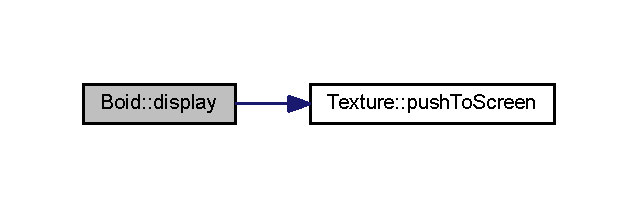
\includegraphics[width=306pt]{class_boid_ad522fbcf60e6e318c785ca7b04091472_cgraph}
\end{center}
\end{figure}


\hypertarget{class_boid_a4f21bfa041637ffcce13c56764fd3c9f}{\index{Boid@{Boid}!get\+Position@{get\+Position}}
\index{get\+Position@{get\+Position}!Boid@{Boid}}
\subsubsection[{get\+Position}]{\setlength{\rightskip}{0pt plus 5cm}{\bf Vec2} Boid\+::get\+Position (
\begin{DoxyParamCaption}
{}
\end{DoxyParamCaption}
)}}\label{class_boid_a4f21bfa041637ffcce13c56764fd3c9f}
Getter \# gets the position \begin{DoxyReturn}{Returns}
\hyperlink{struct_vec2}{Vec2} the position 
\end{DoxyReturn}
\hypertarget{class_boid_a3a5d507c214ebd3bf9eda04e2157c4b5}{\index{Boid@{Boid}!get\+Scale@{get\+Scale}}
\index{get\+Scale@{get\+Scale}!Boid@{Boid}}
\subsubsection[{get\+Scale}]{\setlength{\rightskip}{0pt plus 5cm}{\bf Vec2} Boid\+::get\+Scale (
\begin{DoxyParamCaption}
{}
\end{DoxyParamCaption}
)}}\label{class_boid_a3a5d507c214ebd3bf9eda04e2157c4b5}
Getter \# gets the scale \begin{DoxyReturn}{Returns}
\hyperlink{struct_vec2}{Vec2} the scale 
\end{DoxyReturn}
\hypertarget{class_boid_a3af03753fdadf91e23acd64fb59968c1}{\index{Boid@{Boid}!get\+Velocity@{get\+Velocity}}
\index{get\+Velocity@{get\+Velocity}!Boid@{Boid}}
\subsubsection[{get\+Velocity}]{\setlength{\rightskip}{0pt plus 5cm}{\bf Vec2} Boid\+::get\+Velocity (
\begin{DoxyParamCaption}
{}
\end{DoxyParamCaption}
)}}\label{class_boid_a3af03753fdadf91e23acd64fb59968c1}
Getter \# gets the velocity \begin{DoxyReturn}{Returns}
\hyperlink{struct_vec2}{Vec2} the velocity 
\end{DoxyReturn}
\hypertarget{class_boid_a62ebe99b4a19edfc2d0a6f1ac58e9658}{\index{Boid@{Boid}!set\+Position@{set\+Position}}
\index{set\+Position@{set\+Position}!Boid@{Boid}}
\subsubsection[{set\+Position}]{\setlength{\rightskip}{0pt plus 5cm}void Boid\+::set\+Position (
\begin{DoxyParamCaption}
\item[{{\bf Vec2}}]{in\+Position}
\end{DoxyParamCaption}
)}}\label{class_boid_a62ebe99b4a19edfc2d0a6f1ac58e9658}
Setter \# sets the position 
\begin{DoxyParams}{Parameters}
{\em \hyperlink{struct_vec2}{Vec2}} & the new position \\
\hline
\end{DoxyParams}
\hypertarget{class_boid_a4443fb5d1fb425b9fede21c3cee2ba84}{\index{Boid@{Boid}!set\+Scale@{set\+Scale}}
\index{set\+Scale@{set\+Scale}!Boid@{Boid}}
\subsubsection[{set\+Scale}]{\setlength{\rightskip}{0pt plus 5cm}void Boid\+::set\+Scale (
\begin{DoxyParamCaption}
\item[{{\bf Vec2}}]{in\+Scale}
\end{DoxyParamCaption}
)}}\label{class_boid_a4443fb5d1fb425b9fede21c3cee2ba84}
Setter \# sets the scale 
\begin{DoxyParams}{Parameters}
{\em \hyperlink{struct_vec2}{Vec2}} & the new scale \\
\hline
\end{DoxyParams}
\hypertarget{class_boid_a8f59ceb20ee2f35705ddd1984d98d5c5}{\index{Boid@{Boid}!set\+Velocity@{set\+Velocity}}
\index{set\+Velocity@{set\+Velocity}!Boid@{Boid}}
\subsubsection[{set\+Velocity}]{\setlength{\rightskip}{0pt plus 5cm}void Boid\+::set\+Velocity (
\begin{DoxyParamCaption}
\item[{{\bf Vec2}}]{in\+Velocity}
\end{DoxyParamCaption}
)}}\label{class_boid_a8f59ceb20ee2f35705ddd1984d98d5c5}
Setter \# sets the velocity 
\begin{DoxyParams}{Parameters}
{\em \hyperlink{struct_vec2}{Vec2}} & the new velocity \\
\hline
\end{DoxyParams}


The documentation for this class was generated from the following files\+:\begin{DoxyCompactItemize}
\item 
Flock You!/boid.\+h\item 
Flock You!/boid.\+cpp\end{DoxyCompactItemize}

\hypertarget{class_game}{\section{Game Class Reference}
\label{class_game}\index{Game@{Game}}
}


Creates an \hyperlink{class_game}{Game} object that runs the \hyperlink{class_game}{Game} Creates an \hyperlink{class_game}{Game} object that runs the \hyperlink{class_game}{Game}.  




{\ttfamily \#include $<$game.\+h$>$}

\subsection*{Public Member Functions}
\begin{DoxyCompactItemize}
\item 
\hyperlink{class_game_aa16f7f0fe07387c1fda7f27858b2ff66}{Game} (S\+D\+L\+\_\+\+Renderer $\ast$, int, int)
\item 
\hyperlink{class_game_ae3d112ca6e0e55150d2fdbc704474530}{$\sim$\+Game} ()
\item 
bool \hyperlink{class_game_a6e3ee4ac1c5ee591527cd13cfb4cfab2}{input} ()
\item 
bool \hyperlink{class_game_a34db1b512678bf1bf0bd8e0d56723b18}{update} (float)
\item 
void \hyperlink{class_game_a6d54497ce3a66f6dd45eacfdccc8d0bd}{draw} ()
\end{DoxyCompactItemize}


\subsection{Detailed Description}
Creates an \hyperlink{class_game}{Game} object that runs the \hyperlink{class_game}{Game} Creates an \hyperlink{class_game}{Game} object that runs the \hyperlink{class_game}{Game}. 

\subsection{Constructor \& Destructor Documentation}
\hypertarget{class_game_aa16f7f0fe07387c1fda7f27858b2ff66}{\index{Game@{Game}!Game@{Game}}
\index{Game@{Game}!Game@{Game}}
\subsubsection[{Game}]{\setlength{\rightskip}{0pt plus 5cm}Game\+::\+Game (
\begin{DoxyParamCaption}
\item[{S\+D\+L\+\_\+\+Renderer $\ast$}]{in\+Renderer, }
\item[{int}]{in\+Width, }
\item[{int}]{in\+Height}
\end{DoxyParamCaption}
)}}\label{class_game_aa16f7f0fe07387c1fda7f27858b2ff66}
Constructs an \hyperlink{class_game}{Game} object Constructs the \hyperlink{class_game}{Game} object 
\begin{DoxyParams}{Parameters}
{\em S\+D\+L\+\_\+\+Renderer} & $\ast$ a pointer to the renderer \\
\hline
{\em int} & the screen width \\
\hline
{\em int} & the screen height \\
\hline
\end{DoxyParams}
\hypertarget{class_game_ae3d112ca6e0e55150d2fdbc704474530}{\index{Game@{Game}!````~Game@{$\sim$\+Game}}
\index{````~Game@{$\sim$\+Game}!Game@{Game}}
\subsubsection[{$\sim$\+Game}]{\setlength{\rightskip}{0pt plus 5cm}Game\+::$\sim$\+Game (
\begin{DoxyParamCaption}
{}
\end{DoxyParamCaption}
)}}\label{class_game_ae3d112ca6e0e55150d2fdbc704474530}
De-\/constructs an \hyperlink{class_game}{Game} object De-\/constructs the \hyperlink{class_game}{Game} object 

\subsection{Member Function Documentation}
\hypertarget{class_game_a6d54497ce3a66f6dd45eacfdccc8d0bd}{\index{Game@{Game}!draw@{draw}}
\index{draw@{draw}!Game@{Game}}
\subsubsection[{draw}]{\setlength{\rightskip}{0pt plus 5cm}void Game\+::draw (
\begin{DoxyParamCaption}
{}
\end{DoxyParamCaption}
)}}\label{class_game_a6d54497ce3a66f6dd45eacfdccc8d0bd}
Draws the \hyperlink{class_game}{Game} object \hypertarget{class_game_a6e3ee4ac1c5ee591527cd13cfb4cfab2}{\index{Game@{Game}!input@{input}}
\index{input@{input}!Game@{Game}}
\subsubsection[{input}]{\setlength{\rightskip}{0pt plus 5cm}bool Game\+::input (
\begin{DoxyParamCaption}
{}
\end{DoxyParamCaption}
)}}\label{class_game_a6e3ee4ac1c5ee591527cd13cfb4cfab2}
Handles the game input \begin{DoxyReturn}{Returns}
bool if false the quit game 
\end{DoxyReturn}
\hypertarget{class_game_a34db1b512678bf1bf0bd8e0d56723b18}{\index{Game@{Game}!update@{update}}
\index{update@{update}!Game@{Game}}
\subsubsection[{update}]{\setlength{\rightskip}{0pt plus 5cm}bool Game\+::update (
\begin{DoxyParamCaption}
\item[{float}]{dt}
\end{DoxyParamCaption}
)}}\label{class_game_a34db1b512678bf1bf0bd8e0d56723b18}
Update the \hyperlink{class_game}{Game} object 
\begin{DoxyParams}{Parameters}
{\em float} & the delta\+Time \\
\hline
\end{DoxyParams}
\begin{DoxyReturn}{Returns}
bool if false the quit game 
\end{DoxyReturn}


The documentation for this class was generated from the following files\+:\begin{DoxyCompactItemize}
\item 
Flock You!/game.\+h\item 
Flock You!/game.\+cpp\end{DoxyCompactItemize}

\hypertarget{class_state}{\section{State Class Reference}
\label{class_state}\index{State@{State}}
}


Creates a \hyperlink{class_state}{State} object. Creates a \hyperlink{class_state}{State} object to be inherited.  




{\ttfamily \#include $<$state.\+h$>$}



Inheritance diagram for State\+:\nopagebreak
\begin{figure}[H]
\begin{center}
\leavevmode
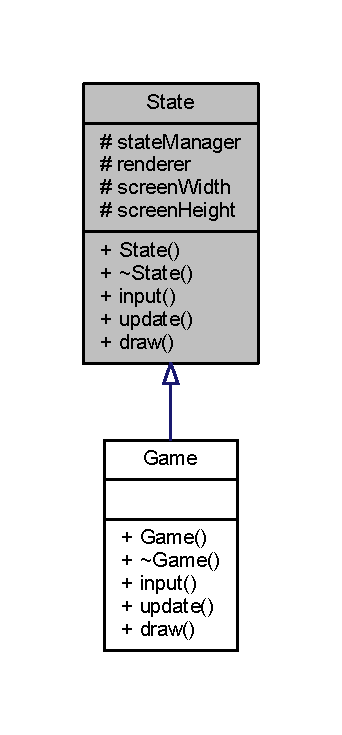
\includegraphics[width=164pt]{class_state__inherit__graph}
\end{center}
\end{figure}


Collaboration diagram for State\+:\nopagebreak
\begin{figure}[H]
\begin{center}
\leavevmode
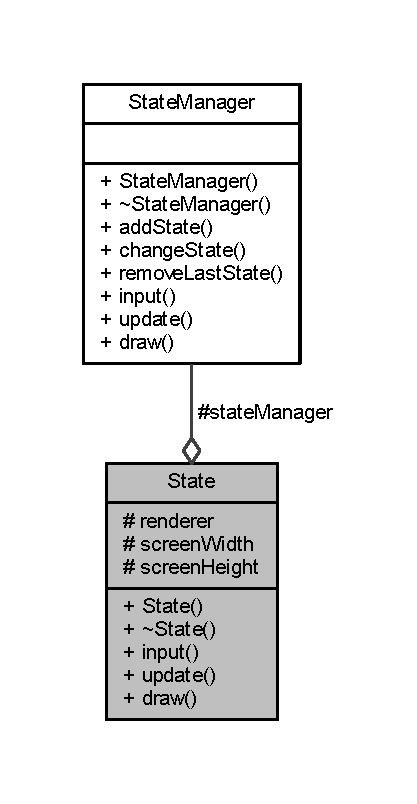
\includegraphics[width=200pt]{class_state__coll__graph}
\end{center}
\end{figure}
\subsection*{Public Member Functions}
\begin{DoxyCompactItemize}
\item 
\hyperlink{class_state_a68fb4089a66325a22f15311356e9df87}{State} (\hyperlink{class_state_manager}{State\+Manager} $\ast$, S\+D\+L\+\_\+\+Renderer $\ast$, int, int)
\item 
virtual \hyperlink{class_state_afab438d92b90dc18d194dbd9c9c8bab3}{$\sim$\+State} ()
\item 
virtual bool \hyperlink{class_state_ac0dcfe3db8d012b37e6935f4f805ece7}{input} ()=0
\item 
virtual void \hyperlink{class_state_a8f582ba039a10fff9712b6a21ef22808}{update} (float delta\+Time)=0
\item 
virtual void \hyperlink{class_state_ae261605bc40b7e3959ce5df5457e4942}{draw} ()=0
\end{DoxyCompactItemize}
\subsection*{Protected Attributes}
\begin{DoxyCompactItemize}
\item 
\hypertarget{class_state_a78388f59b0a570faa4b7ea640fea668e}{\hyperlink{class_state_manager}{State\+Manager} $\ast$ {\bfseries state\+Manager}}\label{class_state_a78388f59b0a570faa4b7ea640fea668e}

\item 
\hypertarget{class_state_ad79f979055823ec66fb7919e90ddd5c9}{S\+D\+L\+\_\+\+Renderer $\ast$ {\bfseries renderer}}\label{class_state_ad79f979055823ec66fb7919e90ddd5c9}

\item 
\hypertarget{class_state_a6fab86df7026a683af0dd9b81eea65c5}{int {\bfseries screen\+Width}}\label{class_state_a6fab86df7026a683af0dd9b81eea65c5}

\item 
\hypertarget{class_state_afd877e4a19f392ed3915b518c49cb68b}{int {\bfseries screen\+Height}}\label{class_state_afd877e4a19f392ed3915b518c49cb68b}

\end{DoxyCompactItemize}


\subsection{Detailed Description}
Creates a \hyperlink{class_state}{State} object. Creates a \hyperlink{class_state}{State} object to be inherited. 

\subsection{Constructor \& Destructor Documentation}
\hypertarget{class_state_a68fb4089a66325a22f15311356e9df87}{\index{State@{State}!State@{State}}
\index{State@{State}!State@{State}}
\subsubsection[{State}]{\setlength{\rightskip}{0pt plus 5cm}State\+::\+State (
\begin{DoxyParamCaption}
\item[{{\bf State\+Manager} $\ast$}]{in\+State\+Manager, }
\item[{S\+D\+L\+\_\+\+Renderer $\ast$}]{in\+Renderer, }
\item[{int}]{in\+Width, }
\item[{int}]{in\+Height}
\end{DoxyParamCaption}
)}}\label{class_state_a68fb4089a66325a22f15311356e9df87}
Constructs a \hyperlink{class_state}{State} object 
\begin{DoxyParams}{Parameters}
{\em \hyperlink{class_state_manager}{State\+Manager}} & $\ast$ a pointer to the \hyperlink{class_state_manager}{State\+Manager} \\
\hline
{\em S\+D\+L\+\_\+\+Renderer} & $\ast$ a pointer to the renderer in use. \\
\hline
{\em int} & the screen width \\
\hline
{\em int} & the screen height \\
\hline
\end{DoxyParams}
\hypertarget{class_state_afab438d92b90dc18d194dbd9c9c8bab3}{\index{State@{State}!````~State@{$\sim$\+State}}
\index{````~State@{$\sim$\+State}!State@{State}}
\subsubsection[{$\sim$\+State}]{\setlength{\rightskip}{0pt plus 5cm}State\+::$\sim$\+State (
\begin{DoxyParamCaption}
{}
\end{DoxyParamCaption}
)\hspace{0.3cm}{\ttfamily [virtual]}}}\label{class_state_afab438d92b90dc18d194dbd9c9c8bab3}
A virtual destructor for the \hyperlink{class_state}{State} object 

\subsection{Member Function Documentation}
\hypertarget{class_state_ae261605bc40b7e3959ce5df5457e4942}{\index{State@{State}!draw@{draw}}
\index{draw@{draw}!State@{State}}
\subsubsection[{draw}]{\setlength{\rightskip}{0pt plus 5cm}virtual void State\+::draw (
\begin{DoxyParamCaption}
{}
\end{DoxyParamCaption}
)\hspace{0.3cm}{\ttfamily [pure virtual]}}}\label{class_state_ae261605bc40b7e3959ce5df5457e4942}
A virtual function to draw to the screen A virtual function to draw to the screen using the renderer 

Implemented in \hyperlink{class_game_a6d54497ce3a66f6dd45eacfdccc8d0bd}{Game}.

\hypertarget{class_state_ac0dcfe3db8d012b37e6935f4f805ece7}{\index{State@{State}!input@{input}}
\index{input@{input}!State@{State}}
\subsubsection[{input}]{\setlength{\rightskip}{0pt plus 5cm}virtual bool State\+::input (
\begin{DoxyParamCaption}
{}
\end{DoxyParamCaption}
)\hspace{0.3cm}{\ttfamily [pure virtual]}}}\label{class_state_ac0dcfe3db8d012b37e6935f4f805ece7}
A virtual function to handle the user input A virtual function to handle the user input for use with the \hyperlink{class_state}{State} \begin{DoxyReturn}{Returns}
bool if false then quit \hyperlink{class_state}{State} 
\end{DoxyReturn}


Implemented in \hyperlink{class_game_a6e3ee4ac1c5ee591527cd13cfb4cfab2}{Game}.

\hypertarget{class_state_a8f582ba039a10fff9712b6a21ef22808}{\index{State@{State}!update@{update}}
\index{update@{update}!State@{State}}
\subsubsection[{update}]{\setlength{\rightskip}{0pt plus 5cm}virtual void State\+::update (
\begin{DoxyParamCaption}
\item[{float}]{delta\+Time}
\end{DoxyParamCaption}
)\hspace{0.3cm}{\ttfamily [pure virtual]}}}\label{class_state_a8f582ba039a10fff9712b6a21ef22808}
A virtual function to update the \hyperlink{class_state}{State} A virtual function to update the \hyperlink{class_state}{State} to allow the \hyperlink{class_state}{State} to run 
\begin{DoxyParams}{Parameters}
{\em float} & the delta time \\
\hline
\end{DoxyParams}


Implemented in \hyperlink{class_game_a419466336fad97182f5051e11f541636}{Game}.



The documentation for this class was generated from the following files\+:\begin{DoxyCompactItemize}
\item 
Flock You!/state.\+h\item 
Flock You!/state.\+cpp\end{DoxyCompactItemize}

\hypertarget{class_state_manager}{\section{State\+Manager Class Reference}
\label{class_state_manager}\index{State\+Manager@{State\+Manager}}
}


Creates a \hyperlink{class_state_manager}{State\+Manager} object. Creates a \hyperlink{class_state_manager}{State\+Manager} object to be inherited.  




{\ttfamily \#include $<$state\+Manager.\+h$>$}



Collaboration diagram for State\+Manager\+:
\nopagebreak
\begin{figure}[H]
\begin{center}
\leavevmode
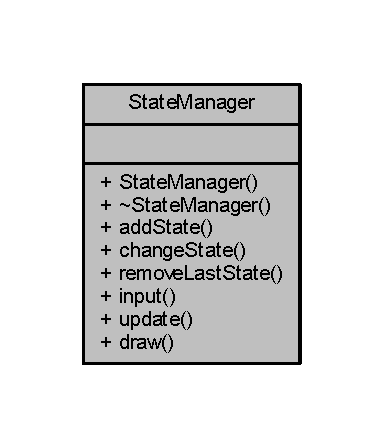
\includegraphics[width=184pt]{class_state_manager__coll__graph}
\end{center}
\end{figure}
\subsection*{Public Member Functions}
\begin{DoxyCompactItemize}
\item 
\hyperlink{class_state_manager_a3e2be96d935eb56813b096a885d58587}{State\+Manager} ()
\item 
\hyperlink{class_state_manager_a05a43504a033f1befad5c5118249ec6f}{$\sim$\+State\+Manager} ()
\item 
void \hyperlink{class_state_manager_a6bc633ce02f7884f082fb4ca1a53639b}{add\+State} (\hyperlink{class_state}{State} $\ast$)
\item 
void \hyperlink{class_state_manager_abad20819be992649c733f45b2a7164e2}{change\+State} (\hyperlink{class_state}{State} $\ast$)
\item 
void \hyperlink{class_state_manager_a9b20b650cab8e9068387ac12b7e60f28}{remove\+Last\+State} ()
\item 
bool \hyperlink{class_state_manager_afa8f2a280c332673075bfdd254a95603}{input} ()
\item 
void \hyperlink{class_state_manager_ae02fb746e1ef597d2842aaec506030b2}{update} (float delta\+Time)
\item 
void \hyperlink{class_state_manager_a22666f2f72320ea3be46e9253b7530e2}{draw} ()
\end{DoxyCompactItemize}


\subsection{Detailed Description}
Creates a \hyperlink{class_state_manager}{State\+Manager} object. Creates a \hyperlink{class_state_manager}{State\+Manager} object to be inherited. 

\subsection{Constructor \& Destructor Documentation}
\hypertarget{class_state_manager_a3e2be96d935eb56813b096a885d58587}{\index{State\+Manager@{State\+Manager}!State\+Manager@{State\+Manager}}
\index{State\+Manager@{State\+Manager}!State\+Manager@{State\+Manager}}
\subsubsection[{State\+Manager}]{\setlength{\rightskip}{0pt plus 5cm}State\+Manager\+::\+State\+Manager (
\begin{DoxyParamCaption}
{}
\end{DoxyParamCaption}
)}}\label{class_state_manager_a3e2be96d935eb56813b096a885d58587}
Constructs a \hyperlink{class_state_manager}{State\+Manager} object \hypertarget{class_state_manager_a05a43504a033f1befad5c5118249ec6f}{\index{State\+Manager@{State\+Manager}!````~State\+Manager@{$\sim$\+State\+Manager}}
\index{````~State\+Manager@{$\sim$\+State\+Manager}!State\+Manager@{State\+Manager}}
\subsubsection[{$\sim$\+State\+Manager}]{\setlength{\rightskip}{0pt plus 5cm}State\+Manager\+::$\sim$\+State\+Manager (
\begin{DoxyParamCaption}
{}
\end{DoxyParamCaption}
)}}\label{class_state_manager_a05a43504a033f1befad5c5118249ec6f}
Destructs a \hyperlink{class_state_manager}{State\+Manager} object 

\subsection{Member Function Documentation}
\hypertarget{class_state_manager_a6bc633ce02f7884f082fb4ca1a53639b}{\index{State\+Manager@{State\+Manager}!add\+State@{add\+State}}
\index{add\+State@{add\+State}!State\+Manager@{State\+Manager}}
\subsubsection[{add\+State}]{\setlength{\rightskip}{0pt plus 5cm}void State\+Manager\+::add\+State (
\begin{DoxyParamCaption}
\item[{{\bf State} $\ast$}]{state}
\end{DoxyParamCaption}
)}}\label{class_state_manager_a6bc633ce02f7884f082fb4ca1a53639b}
Adds a new state Adds a new state to the current stack of states 
\begin{DoxyParams}{Parameters}
{\em \hyperlink{class_state}{State}} & $\ast$ a pointer to the \hyperlink{class_state}{State} in use \\
\hline
\end{DoxyParams}


Here is the caller graph for this function\+:
\nopagebreak
\begin{figure}[H]
\begin{center}
\leavevmode
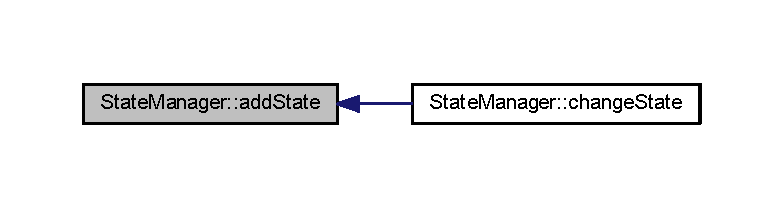
\includegraphics[width=350pt]{class_state_manager_a6bc633ce02f7884f082fb4ca1a53639b_icgraph}
\end{center}
\end{figure}


\hypertarget{class_state_manager_abad20819be992649c733f45b2a7164e2}{\index{State\+Manager@{State\+Manager}!change\+State@{change\+State}}
\index{change\+State@{change\+State}!State\+Manager@{State\+Manager}}
\subsubsection[{change\+State}]{\setlength{\rightskip}{0pt plus 5cm}void State\+Manager\+::change\+State (
\begin{DoxyParamCaption}
\item[{{\bf State} $\ast$}]{state}
\end{DoxyParamCaption}
)}}\label{class_state_manager_abad20819be992649c733f45b2a7164e2}
Changes to a new \hyperlink{class_state}{State} Changes the current \hyperlink{class_state}{State} to a new \hyperlink{class_state}{State} 
\begin{DoxyParams}{Parameters}
{\em \hyperlink{class_state}{State}} & $\ast$ a pointer to the \hyperlink{class_state}{State} in use \\
\hline
\end{DoxyParams}


Here is the call graph for this function\+:
\nopagebreak
\begin{figure}[H]
\begin{center}
\leavevmode
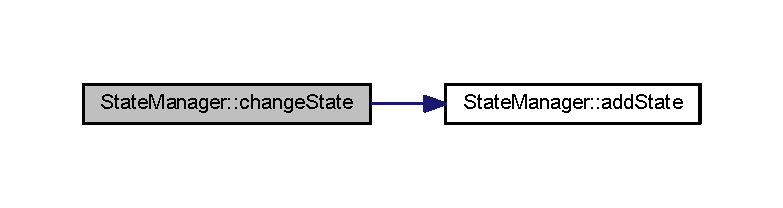
\includegraphics[width=350pt]{class_state_manager_abad20819be992649c733f45b2a7164e2_cgraph}
\end{center}
\end{figure}


\hypertarget{class_state_manager_a22666f2f72320ea3be46e9253b7530e2}{\index{State\+Manager@{State\+Manager}!draw@{draw}}
\index{draw@{draw}!State\+Manager@{State\+Manager}}
\subsubsection[{draw}]{\setlength{\rightskip}{0pt plus 5cm}void State\+Manager\+::draw (
\begin{DoxyParamCaption}
{}
\end{DoxyParamCaption}
)}}\label{class_state_manager_a22666f2f72320ea3be46e9253b7530e2}
Draws the current \hyperlink{class_state}{State} The draw function that will allow the equivalent draw function to run in the current \hyperlink{class_state}{State} \hypertarget{class_state_manager_afa8f2a280c332673075bfdd254a95603}{\index{State\+Manager@{State\+Manager}!input@{input}}
\index{input@{input}!State\+Manager@{State\+Manager}}
\subsubsection[{input}]{\setlength{\rightskip}{0pt plus 5cm}bool State\+Manager\+::input (
\begin{DoxyParamCaption}
{}
\end{DoxyParamCaption}
)}}\label{class_state_manager_afa8f2a280c332673075bfdd254a95603}
Handles the user input The input function that will allow the equivalent input function to run in the current \hyperlink{class_state}{State} \begin{DoxyReturn}{Returns}
bool if false then quit the application 
\end{DoxyReturn}
\hypertarget{class_state_manager_a9b20b650cab8e9068387ac12b7e60f28}{\index{State\+Manager@{State\+Manager}!remove\+Last\+State@{remove\+Last\+State}}
\index{remove\+Last\+State@{remove\+Last\+State}!State\+Manager@{State\+Manager}}
\subsubsection[{remove\+Last\+State}]{\setlength{\rightskip}{0pt plus 5cm}void State\+Manager\+::remove\+Last\+State (
\begin{DoxyParamCaption}
{}
\end{DoxyParamCaption}
)}}\label{class_state_manager_a9b20b650cab8e9068387ac12b7e60f28}
Removes the last \hyperlink{class_state}{State} from the vector \hypertarget{class_state_manager_ae02fb746e1ef597d2842aaec506030b2}{\index{State\+Manager@{State\+Manager}!update@{update}}
\index{update@{update}!State\+Manager@{State\+Manager}}
\subsubsection[{update}]{\setlength{\rightskip}{0pt plus 5cm}void State\+Manager\+::update (
\begin{DoxyParamCaption}
\item[{float}]{delta\+Time}
\end{DoxyParamCaption}
)}}\label{class_state_manager_ae02fb746e1ef597d2842aaec506030b2}
Updates the current \hyperlink{class_state}{State} The update function that will allow the equivalent update function to run in the current \hyperlink{class_state}{State} 
\begin{DoxyParams}{Parameters}
{\em float} & the delta time for use within the update function \\
\hline
\end{DoxyParams}


The documentation for this class was generated from the following files\+:\begin{DoxyCompactItemize}
\item 
Flock You!/state\+Manager.\+h\item 
Flock You!/state\+Manager.\+cpp\end{DoxyCompactItemize}

\hypertarget{class_texture}{\section{Texture Class Reference}
\label{class_texture}\index{Texture@{Texture}}
}


Creates a \hyperlink{class_texture}{Texture} for use with a renderer Creates a \hyperlink{class_texture}{Texture} from an image file, this can then be used with a renderer.  




{\ttfamily \#include $<$texture.\+h$>$}



Collaboration diagram for Texture\+:
\nopagebreak
\begin{figure}[H]
\begin{center}
\leavevmode
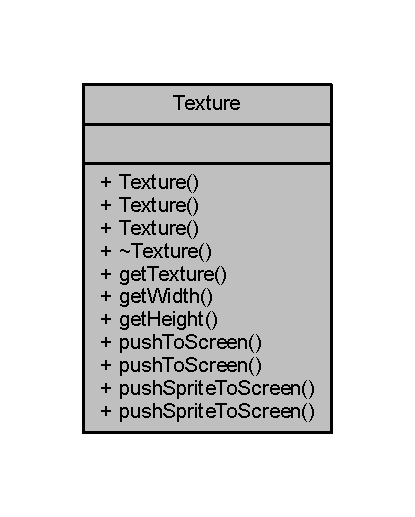
\includegraphics[width=199pt]{class_texture__coll__graph}
\end{center}
\end{figure}
\subsection*{Public Member Functions}
\begin{DoxyCompactItemize}
\item 
\hyperlink{class_texture_a3e603c08f4b2b4f43822a99a6b865bee}{Texture} (S\+D\+L\+\_\+\+Renderer $\ast$, int, int, int)
\item 
\hyperlink{class_texture_a10abeebb644ea969c78f4fa443ec17c1}{Texture} (std\+::string, S\+D\+L\+\_\+\+Renderer $\ast$)
\item 
\hyperlink{class_texture_a6edf59e3b10e474356e8a7878af56b83}{Texture} (std\+::string, S\+D\+L\+\_\+\+Renderer $\ast$, bool)
\item 
\hyperlink{class_texture_a09c4bcb7462f64c1d20fa69dba3cee8a}{$\sim$\+Texture} ()
\item 
S\+D\+L\+\_\+\+Texture $\ast$ \hyperlink{class_texture_a77a1ae0043a4b318a60df3b02ef2d3f6}{get\+Texture} ()
\item 
int \hyperlink{class_texture_a91a6fd3355bc870194851514194daaab}{get\+Width} ()
\item 
int \hyperlink{class_texture_a80e143905655b173df5994300088ce35}{get\+Height} ()
\item 
void \hyperlink{class_texture_aec498f1f84eb10bb60d3c3117884e70f}{push\+To\+Screen} (S\+D\+L\+\_\+\+Renderer $\ast$, int, int)
\item 
void \hyperlink{class_texture_ab3b1f6aa29a50ef2c012fbc9d0cb8bd8}{push\+To\+Screen} (S\+D\+L\+\_\+\+Renderer $\ast$, int, int, int, int)
\item 
void \hyperlink{class_texture_a703db8963b46b751b8affce1807725b7}{push\+Sprite\+To\+Screen} (S\+D\+L\+\_\+\+Renderer $\ast$, int, int, int, int, int, int)
\item 
void \hyperlink{class_texture_a105a3aba66afb7d223ac086aa465b70d}{push\+Sprite\+To\+Screen} (S\+D\+L\+\_\+\+Renderer $\ast$, int, int, int, int, int, int, int, int)
\end{DoxyCompactItemize}


\subsection{Detailed Description}
Creates a \hyperlink{class_texture}{Texture} for use with a renderer Creates a \hyperlink{class_texture}{Texture} from an image file, this can then be used with a renderer. 

\subsection{Constructor \& Destructor Documentation}
\hypertarget{class_texture_a3e603c08f4b2b4f43822a99a6b865bee}{\index{Texture@{Texture}!Texture@{Texture}}
\index{Texture@{Texture}!Texture@{Texture}}
\subsubsection[{Texture}]{\setlength{\rightskip}{0pt plus 5cm}Texture\+::\+Texture (
\begin{DoxyParamCaption}
\item[{S\+D\+L\+\_\+\+Renderer $\ast$}]{renderer, }
\item[{int}]{r, }
\item[{int}]{g, }
\item[{int}]{b}
\end{DoxyParamCaption}
)}}\label{class_texture_a3e603c08f4b2b4f43822a99a6b865bee}
Constructs a \hyperlink{class_texture}{Texture} Creates a \hyperlink{class_texture}{Texture} using an rbg value. This will create a 1x1 rectangle of that colour that can be scaled. 
\begin{DoxyParams}{Parameters}
{\em std\+::string} & The location of the image file. \\
\hline
{\em int} & r \\
\hline
{\em int} & g \\
\hline
{\em int} & b \\
\hline
\end{DoxyParams}
\hypertarget{class_texture_a10abeebb644ea969c78f4fa443ec17c1}{\index{Texture@{Texture}!Texture@{Texture}}
\index{Texture@{Texture}!Texture@{Texture}}
\subsubsection[{Texture}]{\setlength{\rightskip}{0pt plus 5cm}Texture\+::\+Texture (
\begin{DoxyParamCaption}
\item[{std\+::string}]{file\+Name, }
\item[{S\+D\+L\+\_\+\+Renderer $\ast$}]{renderer}
\end{DoxyParamCaption}
)}}\label{class_texture_a10abeebb644ea969c78f4fa443ec17c1}
Constructs a \hyperlink{class_texture}{Texture} Creates a \hyperlink{class_texture}{Texture} using an image location and a renderer. The magenta pixels of this image can represent alpha if needed. This is for use with S\+D\+L image. 
\begin{DoxyParams}{Parameters}
{\em std\+::string} & The location of the image file. \\
\hline
{\em S\+D\+L\+\_\+\+Renderer$\ast$} & The renderer. \\
\hline
\end{DoxyParams}
\hypertarget{class_texture_a6edf59e3b10e474356e8a7878af56b83}{\index{Texture@{Texture}!Texture@{Texture}}
\index{Texture@{Texture}!Texture@{Texture}}
\subsubsection[{Texture}]{\setlength{\rightskip}{0pt plus 5cm}Texture\+::\+Texture (
\begin{DoxyParamCaption}
\item[{std\+::string}]{file\+Name, }
\item[{S\+D\+L\+\_\+\+Renderer $\ast$}]{renderer, }
\item[{bool}]{magenta\+Alpha}
\end{DoxyParamCaption}
)}}\label{class_texture_a6edf59e3b10e474356e8a7878af56b83}
Constructs a \hyperlink{class_texture}{Texture} Creates a \hyperlink{class_texture}{Texture} using an image location and a renderer. The magenta pixels of this image can represent alpha if needed. 
\begin{DoxyParams}{Parameters}
{\em std\+::string} & The location of the image file. \\
\hline
{\em S\+D\+L\+\_\+\+Renderer$\ast$} & The renderer. \\
\hline
{\em bool} & If true any magenta pixels in the image will be converted to alpha \\
\hline
\end{DoxyParams}
\hypertarget{class_texture_a09c4bcb7462f64c1d20fa69dba3cee8a}{\index{Texture@{Texture}!````~Texture@{$\sim$\+Texture}}
\index{````~Texture@{$\sim$\+Texture}!Texture@{Texture}}
\subsubsection[{$\sim$\+Texture}]{\setlength{\rightskip}{0pt plus 5cm}Texture\+::$\sim$\+Texture (
\begin{DoxyParamCaption}
{}
\end{DoxyParamCaption}
)}}\label{class_texture_a09c4bcb7462f64c1d20fa69dba3cee8a}
De-\/constructs a \hyperlink{class_texture}{Texture} De-\/constructs the \hyperlink{class_texture}{Texture} deleting the \hyperlink{class_texture}{Texture} from memory. 

\subsection{Member Function Documentation}
\hypertarget{class_texture_a80e143905655b173df5994300088ce35}{\index{Texture@{Texture}!get\+Height@{get\+Height}}
\index{get\+Height@{get\+Height}!Texture@{Texture}}
\subsubsection[{get\+Height}]{\setlength{\rightskip}{0pt plus 5cm}int Texture\+::get\+Height (
\begin{DoxyParamCaption}
{}
\end{DoxyParamCaption}
)}}\label{class_texture_a80e143905655b173df5994300088ce35}
Getter \# Returns texture\+Height Returns the value of texture\+Height. \hypertarget{class_texture_a77a1ae0043a4b318a60df3b02ef2d3f6}{\index{Texture@{Texture}!get\+Texture@{get\+Texture}}
\index{get\+Texture@{get\+Texture}!Texture@{Texture}}
\subsubsection[{get\+Texture}]{\setlength{\rightskip}{0pt plus 5cm}S\+D\+L\+\_\+\+Texture $\ast$ Texture\+::get\+Texture (
\begin{DoxyParamCaption}
{}
\end{DoxyParamCaption}
)}}\label{class_texture_a77a1ae0043a4b318a60df3b02ef2d3f6}
Getter \# Returns a pointer to the \hyperlink{class_texture}{Texture} Returns a pointer to the \hyperlink{class_texture}{Texture} data. \hypertarget{class_texture_a91a6fd3355bc870194851514194daaab}{\index{Texture@{Texture}!get\+Width@{get\+Width}}
\index{get\+Width@{get\+Width}!Texture@{Texture}}
\subsubsection[{get\+Width}]{\setlength{\rightskip}{0pt plus 5cm}int Texture\+::get\+Width (
\begin{DoxyParamCaption}
{}
\end{DoxyParamCaption}
)}}\label{class_texture_a91a6fd3355bc870194851514194daaab}
Getter \# Returns texture\+Width Returns the value of texture\+Width. \hypertarget{class_texture_a703db8963b46b751b8affce1807725b7}{\index{Texture@{Texture}!push\+Sprite\+To\+Screen@{push\+Sprite\+To\+Screen}}
\index{push\+Sprite\+To\+Screen@{push\+Sprite\+To\+Screen}!Texture@{Texture}}
\subsubsection[{push\+Sprite\+To\+Screen}]{\setlength{\rightskip}{0pt plus 5cm}void Texture\+::push\+Sprite\+To\+Screen (
\begin{DoxyParamCaption}
\item[{S\+D\+L\+\_\+\+Renderer $\ast$}]{renderer, }
\item[{int}]{x, }
\item[{int}]{y, }
\item[{int}]{src\+X, }
\item[{int}]{src\+Y, }
\item[{int}]{src\+Width, }
\item[{int}]{src\+Height}
\end{DoxyParamCaption}
)}}\label{class_texture_a703db8963b46b751b8affce1807725b7}
Pushes the image to the Renderer, to the X\+Y Coordinates. Only displays the source rectangle inputed. 
\begin{DoxyParams}{Parameters}
{\em S\+D\+L\+\_\+\+Renderer$\ast$} & The renderer. \\
\hline
{\em int} & x coordinate of the image. \\
\hline
{\em int} & y coordinate of the image. \\
\hline
{\em int} & x coordinate of the source image. \\
\hline
{\em int} & y coordinate of the source image. \\
\hline
{\em int} & width of the source image. \\
\hline
{\em int} & height of the source image. \\
\hline
\end{DoxyParams}
\hypertarget{class_texture_a105a3aba66afb7d223ac086aa465b70d}{\index{Texture@{Texture}!push\+Sprite\+To\+Screen@{push\+Sprite\+To\+Screen}}
\index{push\+Sprite\+To\+Screen@{push\+Sprite\+To\+Screen}!Texture@{Texture}}
\subsubsection[{push\+Sprite\+To\+Screen}]{\setlength{\rightskip}{0pt plus 5cm}void Texture\+::push\+Sprite\+To\+Screen (
\begin{DoxyParamCaption}
\item[{S\+D\+L\+\_\+\+Renderer $\ast$}]{renderer, }
\item[{int}]{x, }
\item[{int}]{y, }
\item[{int}]{src\+X, }
\item[{int}]{src\+Y, }
\item[{int}]{src\+Width, }
\item[{int}]{src\+Height, }
\item[{int}]{width, }
\item[{int}]{height}
\end{DoxyParamCaption}
)}}\label{class_texture_a105a3aba66afb7d223ac086aa465b70d}
Pushes the image to the Renderer, to the X\+Y Coordinates. Only displays the source rectangle inputed. This is scaled to the width and height inputed. 
\begin{DoxyParams}{Parameters}
{\em S\+D\+L\+\_\+\+Renderer$\ast$} & The renderer. \\
\hline
{\em int} & x coordinate of the image. \\
\hline
{\em int} & y coordinate of the image. \\
\hline
{\em int} & x coordinate of the source image. \\
\hline
{\em int} & y coordinate of the source image. \\
\hline
{\em int} & width of the source image. \\
\hline
{\em int} & height of the source image. \\
\hline
{\em int} & width of the scaled image. \\
\hline
{\em int} & height of the scaled image. \\
\hline
\end{DoxyParams}
\hypertarget{class_texture_aec498f1f84eb10bb60d3c3117884e70f}{\index{Texture@{Texture}!push\+To\+Screen@{push\+To\+Screen}}
\index{push\+To\+Screen@{push\+To\+Screen}!Texture@{Texture}}
\subsubsection[{push\+To\+Screen}]{\setlength{\rightskip}{0pt plus 5cm}void Texture\+::push\+To\+Screen (
\begin{DoxyParamCaption}
\item[{S\+D\+L\+\_\+\+Renderer $\ast$}]{renderer, }
\item[{int}]{x, }
\item[{int}]{y}
\end{DoxyParamCaption}
)}}\label{class_texture_aec498f1f84eb10bb60d3c3117884e70f}
Pushes the image to the Renderer, to the X\+Y Coordinates. 
\begin{DoxyParams}{Parameters}
{\em S\+D\+L\+\_\+\+Renderer$\ast$} & The renderer. \\
\hline
{\em int} & x coordinate of the image. \\
\hline
{\em int} & y coordinate of the image. \\
\hline
\end{DoxyParams}


Here is the caller graph for this function\+:
\nopagebreak
\begin{figure}[H]
\begin{center}
\leavevmode
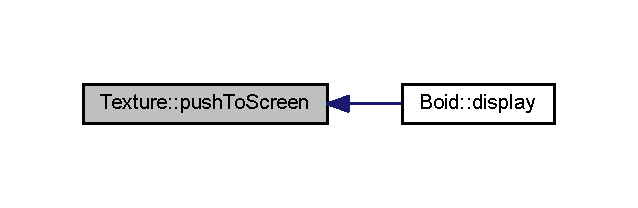
\includegraphics[width=306pt]{class_texture_aec498f1f84eb10bb60d3c3117884e70f_icgraph}
\end{center}
\end{figure}


\hypertarget{class_texture_ab3b1f6aa29a50ef2c012fbc9d0cb8bd8}{\index{Texture@{Texture}!push\+To\+Screen@{push\+To\+Screen}}
\index{push\+To\+Screen@{push\+To\+Screen}!Texture@{Texture}}
\subsubsection[{push\+To\+Screen}]{\setlength{\rightskip}{0pt plus 5cm}void Texture\+::push\+To\+Screen (
\begin{DoxyParamCaption}
\item[{S\+D\+L\+\_\+\+Renderer $\ast$}]{renderer, }
\item[{int}]{x, }
\item[{int}]{y, }
\item[{int}]{width, }
\item[{int}]{height}
\end{DoxyParamCaption}
)}}\label{class_texture_ab3b1f6aa29a50ef2c012fbc9d0cb8bd8}
Pushes the image to the Renderer, to the X\+Y Coordinates. This is scaled to the width and height inputed. 
\begin{DoxyParams}{Parameters}
{\em S\+D\+L\+\_\+\+Renderer$\ast$} & The renderer. \\
\hline
{\em int} & x coordinate of the image. \\
\hline
{\em int} & y coordinate of the image. \\
\hline
{\em int} & width of the scaled image. \\
\hline
{\em int} & height of the scaled image. \\
\hline
\end{DoxyParams}


The documentation for this class was generated from the following files\+:\begin{DoxyCompactItemize}
\item 
Flock You!/texture.\+h\item 
Flock You!/texture.\+cpp\end{DoxyCompactItemize}

\hypertarget{struct_vec2}{\section{Vec2 Struct Reference}
\label{struct_vec2}\index{Vec2@{Vec2}}
}


Creates an \hyperlink{struct_vec2}{Vec2} structure with functions Creates an \hyperlink{struct_vec2}{Vec2} structure with overloaded operators to create a new variable type for use as a 2\+D vector.  




{\ttfamily \#include $<$vec2.\+h$>$}



Collaboration diagram for Vec2\+:\nopagebreak
\begin{figure}[H]
\begin{center}
\leavevmode
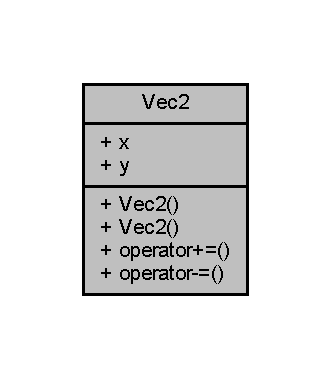
\includegraphics[width=159pt]{struct_vec2__coll__graph}
\end{center}
\end{figure}
\subsection*{Public Member Functions}
\begin{DoxyCompactItemize}
\item 
\hyperlink{struct_vec2_a76080feed7005893ecc634f903cfbae0}{Vec2} ()
\item 
\hyperlink{struct_vec2_a08e2e10202361659c3b7d003ee84ebec}{Vec2} (float input\+X, float input\+Y)
\item 
\hyperlink{struct_vec2}{Vec2} $\ast$ \hyperlink{struct_vec2_a00055ba3b91ef5faeaeb12a4289572f6}{operator+=} (\hyperlink{struct_vec2}{Vec2} a)
\item 
\hyperlink{struct_vec2}{Vec2} $\ast$ \hyperlink{struct_vec2_a6171d807b945b23574c33d6ddf1af74a}{operator-\/=} (\hyperlink{struct_vec2}{Vec2} a)
\end{DoxyCompactItemize}
\subsection*{Public Attributes}
\begin{DoxyCompactItemize}
\item 
\hypertarget{struct_vec2_adf8ee322d4b4bcc04146762c018d731f}{float {\bfseries x}}\label{struct_vec2_adf8ee322d4b4bcc04146762c018d731f}

\item 
\hypertarget{struct_vec2_a30543787e62f6d915543cf1dfb04c094}{float {\bfseries y}}\label{struct_vec2_a30543787e62f6d915543cf1dfb04c094}

\end{DoxyCompactItemize}


\subsection{Detailed Description}
Creates an \hyperlink{struct_vec2}{Vec2} structure with functions Creates an \hyperlink{struct_vec2}{Vec2} structure with overloaded operators to create a new variable type for use as a 2\+D vector. 

\subsection{Constructor \& Destructor Documentation}
\hypertarget{struct_vec2_a76080feed7005893ecc634f903cfbae0}{\index{Vec2@{Vec2}!Vec2@{Vec2}}
\index{Vec2@{Vec2}!Vec2@{Vec2}}
\subsubsection[{Vec2}]{\setlength{\rightskip}{0pt plus 5cm}Vec2\+::\+Vec2 (
\begin{DoxyParamCaption}
{}
\end{DoxyParamCaption}
)\hspace{0.3cm}{\ttfamily [inline]}}}\label{struct_vec2_a76080feed7005893ecc634f903cfbae0}
Constructs an \hyperlink{struct_vec2}{Vec2} Constructs the \hyperlink{struct_vec2}{Vec2} setting the values to 0,0 \hypertarget{struct_vec2_a08e2e10202361659c3b7d003ee84ebec}{\index{Vec2@{Vec2}!Vec2@{Vec2}}
\index{Vec2@{Vec2}!Vec2@{Vec2}}
\subsubsection[{Vec2}]{\setlength{\rightskip}{0pt plus 5cm}Vec2\+::\+Vec2 (
\begin{DoxyParamCaption}
\item[{float}]{input\+X, }
\item[{float}]{input\+Y}
\end{DoxyParamCaption}
)\hspace{0.3cm}{\ttfamily [inline]}}}\label{struct_vec2_a08e2e10202361659c3b7d003ee84ebec}
Constructs a \hyperlink{struct_vec2}{Vec2} Constructs the \hyperlink{struct_vec2}{Vec2} setting the values to the input coordinates 
\begin{DoxyParams}{Parameters}
{\em float} & The inputed x position \\
\hline
{\em float} & The inputed y position \\
\hline
\end{DoxyParams}


\subsection{Member Function Documentation}
\hypertarget{struct_vec2_a00055ba3b91ef5faeaeb12a4289572f6}{\index{Vec2@{Vec2}!operator+=@{operator+=}}
\index{operator+=@{operator+=}!Vec2@{Vec2}}
\subsubsection[{operator+=}]{\setlength{\rightskip}{0pt plus 5cm}{\bf Vec2}$\ast$ Vec2\+::operator+= (
\begin{DoxyParamCaption}
\item[{{\bf Vec2}}]{a}
\end{DoxyParamCaption}
)\hspace{0.3cm}{\ttfamily [inline]}}}\label{struct_vec2_a00055ba3b91ef5faeaeb12a4289572f6}
Overloads the += operator Overloads the += operator allowing a \hyperlink{struct_vec2}{Vec2} variable to use += 
\begin{DoxyParams}{Parameters}
{\em \hyperlink{struct_vec2}{Vec2}} & The input \hyperlink{struct_vec2}{Vec2} \\
\hline
\end{DoxyParams}
\hypertarget{struct_vec2_a6171d807b945b23574c33d6ddf1af74a}{\index{Vec2@{Vec2}!operator-\/=@{operator-\/=}}
\index{operator-\/=@{operator-\/=}!Vec2@{Vec2}}
\subsubsection[{operator-\/=}]{\setlength{\rightskip}{0pt plus 5cm}{\bf Vec2}$\ast$ Vec2\+::operator-\/= (
\begin{DoxyParamCaption}
\item[{{\bf Vec2}}]{a}
\end{DoxyParamCaption}
)\hspace{0.3cm}{\ttfamily [inline]}}}\label{struct_vec2_a6171d807b945b23574c33d6ddf1af74a}
Overloads the -\/= operator Overloads the -\/= operator allowing a \hyperlink{struct_vec2}{Vec2} variable to use -\/= 
\begin{DoxyParams}{Parameters}
{\em \hyperlink{struct_vec2}{Vec2}} & The input \hyperlink{struct_vec2}{Vec2} \\
\hline
\end{DoxyParams}


The documentation for this struct was generated from the following file\+:\begin{DoxyCompactItemize}
\item 
Flock You!/vec2.\+h\end{DoxyCompactItemize}

%--- End generated contents ---

% Index
\newpage
\phantomsection
\addcontentsline{toc}{chapter}{Index}
\printindex

\end{document}
